\chapter{Self-Calibrating Control Layer for Heterogeneous Trackers}\label{ch:layer}

This chapter addresses the second research question: whether a training-free layer placed between a frozen detector and a frozen tracker can keep published trackers operating when the detector's confidence scale changes or becomes noisy, while leaving well-matched pipelines unchanged. The chapter is based on the journal manuscript [P3] listed in the front matter; this chapter gives the complete design history, ablation, and runtime analysis.

\section{Overview}\label{sec:ch5-overview}
In an engineered tracking system the detector and the tracker are rarely developed together. A detector is replaced by a faster or more accurate model, retrained for a new sensor, or quantized for an embedded processor, while the tracker keeps the thresholds its authors tuned for another detector. The confidence scale of the new detector is generally different \cite{kuppers2020detcalib}, and nothing in the pipeline notices. The consequences are large and silent: in the experiments of this chapter, rescaling the confidence of a published detector by one half drives two well-known trackers from about 67 to 0 HOTA, because no detection reaches their fixed thresholds, and a cubic reshaping of the same scores costs them about 7 and 8 points. Retuning every tracker for every detector requires labelled data from the deployment domain, which an operational system lacks.

The layer studied here removes that dependence without retraining or retuning. It sits between a frozen detector and a frozen tracker. At every frame it estimates, from the recent stream of detector scores alone, how the scores separate into background, ambiguous, and confident candidates; decides whether the stream is clean enough to leave the tracker alone; and, when it is not, selects which candidates reach the tracker, remaps their scores, and moves the tracker's association and birth thresholds. It also supplies a track-continuation stage to trackers that lack one. The layer reads the tracker's declared operating point, called its host contract, but contains no detector, tracker, dataset, or sequence names. In the repository of this work, the frozen configuration is named V7f; the name is used in some tables of this chapter.

The contributions of the chapter are the layer itself, the host contract that makes it applicable to single-stage, two-stage, coordinate-only, and two-view trackers, the development and freeze protocol of Sec.~\ref{sec:m-protocol} applied to it, and an evaluation of one frozen configuration on nine published trackers (a tenth failed reproduction), four sources of detections, and three datasets. The layer was designed to be detector- and tracker-agnostic and is evaluated on a heterogeneous set of published systems. The chapter does not claim that it improves every tracker: on clean, well-matched pipelines it is designed to do nothing, and it does nothing.

\section{From Scene-Driven to Score-Driven Control}\label{sec:ch5-scene}
The controller of Chapter~\ref{ch:scene} reads the scene, namely its density, texture, illumination, and blur, and sets the detector's operating point accordingly, in the spirit of content-adaptive video analytics \cite{jiang2018chameleon}. Chapter~\ref{ch:scene} showed that its benefit came from calibration rather than from switching, and its cue audit (Sec.~\ref{sec:ch4-cueaudit}) showed that the image cues did not identify the frames in which a different operating point helps, whereas cues describing the detector output did carry signal. Such scene-driven control also has three structural limitations for heterogeneous pipelines. First, its cue scale and its mapping to thresholds are defined for one detector: the same scene produces different score distributions under different detectors, so a threshold chosen from scene cues is only valid for the detector it was calibrated with. Second, it cannot observe the failure mode that matters most when components are exchanged, namely a shift of the detector's confidence scale, because that shift leaves the image unchanged. Third, it acts on the detector, whereas the thresholds that fail are the tracker's. The layer of this paper therefore reads the detector's scores rather than the image, and it acts on the tracker's input and thresholds rather than on the detector.

\section{Problem Formulation}\label{sec:ch5-problem}
At frame $t$ a frozen detector emits candidates $\{(\mathbf{x}_i, s_i, c_i)\}$ with boxes $\mathbf{x}_i$, scores $s_i\in(0,1)$, and class labels $c_i$, down to an emission floor. A frozen tracker declares a host contract $(a, b, \ell, m_0)$: the score threshold of its first association, the lowest score from which a new track can start, the lowest score any of its association stages uses, and its matching tolerance. A single-stage tracker has $\ell=\min(a,b)$; a two-stage tracker has $\ell<\min(a,b)$. The layer $\mathcal{L}$ outputs, per frame, the subset of candidates passed to the tracker, the scores passed with them, and the thresholds $(a_t, b_t)$ and tolerance $m_t$ the tracker uses at that frame:
\begin{equation}
\left(K_t, \tilde s_{K_t}, a_t, b_t, m_t\right) = \mathcal{L}\left(\{z_i\}_{<t}, \{(\mathbf{x}_i, s_i, c_i)\}_t, \mathcal{T}_{t-1}, g_t;\; a,b,\ell,m_0\right),
\label{eq:ch5-layer}
\end{equation}
where $\{z_i\}_{<t}$ are the logits of earlier frames, $\mathcal{T}_{t-1}$ are the tracker's output tracks of the previous frame, and $g_t$ is an optional scalar image-motion cue of frame $t$. The layer is causal: statistics use frames before $t$ only, and frame-$t$ data enter its state after the decision.

The requirements are that (i) the layer needs no training or dataset-specific labelled calibration, (ii) one frozen configuration is used for every tracker, detector, and dataset, (iii) the output is unchanged when the tracker's operating point already fits the stream, and (iv) the cost per frame is small relative to the detector.

\section{Universal Control Architecture}\label{sec:ch5-arch}
Figure~\ref{fig:ch5-arch} shows the layer. It has four parts: stream statistics, a regime estimate, a regime-dependent candidate policy, and a track-continuation rescue. The configuration of every part is frozen (Sec.~\ref{sec:ch5-protocol}).

\begin{figure}[tbp]
\centering
\resizebox{\textwidth}{!}{%
\begin{tikzpicture}[
  box/.style={draw, rounded corners=2pt, align=center, font=\small, minimum height=10mm, minimum width=22mm, inner sep=3pt},
  arr/.style={-{Stealth[length=2.2mm]}, thick}, lab/.style={font=\scriptsize}]
\node[box] (det) at (0,0) {Frozen\\detector};
\node[box] (pol) at (4.9,0) {Candidate policy\\(clean or noisy)};
\node[box] (res) at (9.6,0) {Continuation\\rescue};
\node[box] (trk) at (14.1,0) {Frozen\\tracker};
\node[box] (stat) at (0,-2.4) {Stream statistics:\\nested Otsu on logits\\of frames $t-W..t-1$};
\node[box] (reg) at (4.9,-2.4) {Regime estimate\\clean if $\bar\rho_t \ge \tfrac12$};
\node[box] (hc) at (11.85,-2.4) {Host contract\\$(a, b, \ell, m_0)$};
\draw[arr] (det) -- node[lab, above]{candidates} (pol);
\draw[arr] (pol) -- (res);
\draw[arr] (res) -- node[lab, above]{$K_t$, scores} (trk);
\draw[arr] (det) -- (stat);
\draw[arr] (stat) -- node[lab, above]{$t_1, t_2, \rho$} (reg);
\draw[arr] (reg) -- (pol);
\draw[arr] (hc.north) ++(-0.6,0) |- ++(0,0.5) -| (res.south);
\draw[arr] (hc.north) ++(0.6,0) |- ++(0,0.5) -| node[lab, pos=0.75, right]{$a_t, b_t, m_t$} (trk.south);
\draw[arr] (trk.north) -- ++(0,0.5) -| node[lab, pos=0.25, above]{tracks of frame $t-1$} (res.north);
\end{tikzpicture}}
\caption{Self-calibrating control layer between a frozen detector and a frozen tracker. Statistics use earlier frames only; the host contract is the tracker's published operating point; the tracker receives the selected candidates, their scores, and its thresholds for the frame.}
\label{fig:ch5-arch}
\end{figure}

\section{Causal Self-Calibration}\label{sec:ch5-calib}
The layer pools the logits of all candidates of the previous $W=10$ frames and splits them twice with the exact Otsu threshold \cite{otsu1979}: the first split $t_1$ separates background from foreground, and a second split of the foreground, $t_2$, separates ambiguous from confident candidates. The confident share of the foreground,
\begin{equation}
\rho_t = \frac{\left|\{i: z_i \ge t_2\}\right|}{\left|\{i: z_i \ge t_1\}\right|},
\label{eq:ch5-rho}
\end{equation}
summarizes how cleanly the detector separates objects from clutter. Working on logits makes the splits invariant to affine transforms of the logit, such as a change of temperature; the host's thresholds are compared on the same scale.

The bands are interpretable only if the stream has a background mode. When the class below $t_1$ holds fewer pooled candidates than the foreground, which happens when a detector emits few low-scoring candidates, the first split falls inside the objects and $\rho$ would falsely signal clutter. In that case the frame counts as clean evidence ($\rho_t=1$). This interpretability check was added after a development diagnosis in which sequence starts with about ten candidates per frame produced splits at $t_1\approx0.6$ and $t_2\approx0.93$ in probability terms and a false noisy call.

\section{Intervention Regimes}\label{sec:ch5-regimes}

\subsection{Regime estimate}
The stream is clean at frame $t$ if the median $\bar\rho_t$ of $\rho$ over all past non-cold frames is at least one half; otherwise it is noisy. The regime is thus a property of the detector and scene stream rather than of a single frame, so that a transient confidence dip, for example under fast camera motion, does not flip it. Before the first valid split (the first frame of a stream), the regime is cold.

\subsection{Cold and clean regimes: self-limiting}
In the cold and clean regimes the tracker's own thresholds are kept, and they are lowered only as far as $t_2$ when the tracker would otherwise reject the confident class: $a_t=\min(a, \sigma(t_2))$ and likewise for $b_t$, where $\sigma$ is the logistic function. Scores are passed unchanged, and only cross-class duplicates, that is, one box proposed with two class labels, are removed. On a stream whose confident class lies above the tracker's thresholds, the tracker therefore receives exactly its native input.

\subsection{Noisy regime: banded intervention}
In the noisy regime the candidates are banded: the primary band $z\ge t_2$ may start and continue tracks, the extension band $t_1\le z<t_2$ may continue tracks but not start them, and candidates below $t_1$ are discarded. Scores are remapped through their empirical distribution in the stream, primary candidates to $[0.5,1)$ and extension candidates to $[0.1,0.5)$, and the tracker's association and birth thresholds are set to 0.5, so that extension candidates can reach only a tracker's low stage. Duplicates are resolved with track context: a weaker candidate overlapping a stronger one (overlap above one half) is removed unless a different track of the previous frame claims it, which keeps occluded people in crowds.

\subsection{Continuation rescue}
A foreground candidate ($z\ge t_1$; every emitted candidate when the stream has no background mode) that continues an existing track of frame $t-1$ with overlap at least one half, where no usable candidate covers that track and the tracker could not see the candidate at the operating point passed this frame, is passed to the tracker with its score raised just above the lowest threshold the tracker uses at that frame. For a two-stage tracker this band is empty by construction because $\ell$ already admits such candidates; for a single-stage tracker it supplies the continuation stage the tracker lacks.

\subsection{Motion rule}
In noisy frames only, and only when an image-motion cue is available, the matching tolerance widens with the ratio $r_t$ of the current global image motion (phase correlation on a quarter-resolution frame \cite{reddy1996phasecorr}) to its past median:
\begin{equation}
m_t=\min\left(0.95,\; 1-\frac{1-m_0}{\max(1,r_t)}\right).
\label{eq:ch5-motion}
\end{equation}


\subsection{Per-frame decision}
Algorithm~\ref{alg:ch5-layer} summarizes the decision of the layer for one frame. Every statistic that decides the regime and the thresholds is computed from earlier frames; the logits of frame $t$ enter the buffer only after the decision.

\begin{algorithm}[tbp]
\caption{Per-frame decision of the self-calibrating control layer (frozen configuration).}
\label{alg:ch5-layer}
\small
\begin{algorithmic}[1]
\Require candidates $\{(\mathbf{x}_i,s_i,c_i)\}$ of frame $t$; logit buffer $H$ of frames $t-W,\ldots,t-1$; history $R$ of $\rho$; tracks $\mathcal{T}_{t-1}$; host contract $(a,b,\ell,m_0)$; optional motion ratio $r_t$
\Ensure passed candidates $K_t$, their scores, thresholds $a_t, b_t$, tolerance $m_t$
\If{$H$ admits no valid split}
  \State regime $\gets$ cold;\quad $(a_t,b_t)\gets(a,b)$
\Else
  \State $t_1 \gets \mathrm{Otsu}(H)$;\quad $t_2 \gets \mathrm{Otsu}(\{z\in H: z\ge t_1\})$
  \State $\rho_t \gets |\{z\in H: z\ge t_2\}| \,/\, |\{z\in H: z\ge t_1\}|$
  \If{$|\{z\in H: z<t_1\}| < |\{z\in H: z\ge t_1\}|$} \Comment{no background mode}
    \State $\rho_t \gets 1$
  \EndIf
  \State append $\rho_t$ to $R$;\quad $\bar\rho_t \gets \mathrm{median}(R)$
  \If{$\bar\rho_t \ge 1/2$}
    \State regime $\gets$ clean;\quad $a_t \gets \min(a,\sigma(t_2))$;\quad $b_t \gets \min(b,\sigma(t_2))$
  \Else
    \State regime $\gets$ noisy;\quad discard candidates with $z_i<t_1$
    \State remap scores by their stream ECDF: $z_i\ge t_2 \mapsto [0.5,1)$, $t_1\le z_i<t_2 \mapsto [0.1,0.5)$
    \State $a_t \gets 0.5$;\quad $b_t \gets 0.5$
  \EndIf
\EndIf
\If{regime is noisy}
  \State remove weaker overlapping candidates (IoU $>0.5$) unless a different track of $\mathcal{T}_{t-1}$ claims them
\Else
  \State remove cross-class duplicates only; pass scores unchanged
\EndIf
\ForAll{tracks $\tau\in\mathcal{T}_{t-1}$ not covered by a usable candidate}
  \State pass the strongest foreground candidate with IoU $\ge 0.5$ to $\tau$ that the tracker cannot see this frame, with its score raised just above the lowest threshold the tracker uses
\EndFor
\State $m_t \gets m_0$;\quad \textbf{if} regime is noisy and $r_t$ is available \textbf{then} $m_t \gets \min\!\left(0.95,\,1-(1-m_0)/\max(1,r_t)\right)$
\State append the logits of frame $t$ to $H$ and drop frames older than $t-W+1$
\end{algorithmic}
\end{algorithm}

\section{Host Contract and Adapters}\label{sec:ch5-contract}
Table~\ref{tab:ch5-contracts} lists the contracts used. Each value is a documented property of the published tracker configuration, not a fitted quantity. An adapter per tracker family maps the layer's decision onto the tracker's interface: the selected candidates and their scores replace the detector output of the frame, and the thresholds and tolerance replace the tracker's own for that frame. Where a tracker has no overlap gate (C-TWiX) or two detection views (TrackTrack), the adapter maps only what the tracker exposes; in TrackTrack's second view a detection that matches a candidate at overlap 0.97 or more, the tracker's own rule, follows that candidate. Post-processing that the authors apply after tracking (interpolation, offline linking) is kept unchanged and evaluated as in the original papers. Tracker-agnostic is meant in this sense: the policy and all of its parameters are identical for every tracker, a tracker enters only through its published contract values, and the adapter translates the decision without making one.

\begin{table}[tbp]
\centering
\caption{Host contracts: the operating point each published tracker declares, as used by the layer. $\tau$ is the tracker's own published threshold, which differs between trackers and, for TrackTrack, between sequences.}
\label{tab:ch5-contracts}
\small\setlength{\tabcolsep}{4pt}
\begin{adjustbox}{max width=\textwidth}
\begin{tabular}{>{\raggedright\arraybackslash}p{3.4cm}ccccc>{\raggedright\arraybackslash}p{3.6cm}}
\hline
Tracker (setting) & Type & assoc & birth & low & match & Decision mapped to \\
\hline
ByteTrack (official MOT17) & two-stage & 0.6 & 0.7 & 0.1 & 0.8 & thresholds, candidates, scores \\
ByteTrack (library default) & two-stage & 0.25 & 0.25 & 0.1 & 0.8 & same \\
SparseTrack & two-stage & $\tau$ & $\tau+0.1$ & 0.1 & published & same \\
BoostTrack & two-stage & $\tau$ & $\tau$ & 0.1 & $1-$IoU gate & same \\
Hybrid-SORT & two-stage & $\tau$ & $\tau$ & 0.1 & $1-$IoU gate & same \\
OC-SORT & single-stage & 0.6 & 0.6 & 0.6 & 0.7 & same \\
PD-SORT & single-stage & $\tau$ & $\tau$ & $\tau$ & $1-$IoU gate & same \\
C-TWiX (MOT17 / KITTI / DanceTrack) & single-stage & 0.5 & 0.7 / 0.5 / 0.9 & 0.5 & not mapped & candidates, scores, two score thresholds \\
TrackTrack & two-view & $\tau_{\mathrm{det}}$ & $\tau_{\mathrm{init}}$ & 0.1 & not mapped & candidates in both views, two thresholds \\
\hline
\end{tabular}
\end{adjustbox}
\end{table}


\section{Complexity}\label{sec:ch5-complexity}
Per frame the layer sorts the pooled logits of at most $W$ frames for the two Otsu splits, computes candidate overlaps with the candidates and with the previous frame's tracks, and, when the motion cue is used, computes one phase correlation on a quarter-resolution image. With $n$ candidates per frame and $k$ tracks, the cost is $O(Wn\log(Wn) + n^2 + nk)$ plus the fixed image cost. The state is a ring buffer of $W$ frames of logits and a history of 100 motion ratios.

\section{Development and Freeze Protocol}\label{sec:ch5-protocol}

\subsection{Design history}
The layer evolved from an earlier design of the same research program that always intervened: it banded the stream with the same thresholds, removed every overlapping duplicate, and remapped scores in every frame. That design helped with miscalibrated and noisy detectors but hurt strong published trackers: on MOT17 it cost SparseTrack 4.15 HOTA points ($[-5.54,-1.66]$) and BoostTrack 5.89 points ($[-7.76,-2.87]$), because overlap-based duplicate removal deleted occluded people in crowds and its self-calibrated thresholds were stricter than the trackers' own (false positives fell by 1,630 and 1,351, false negatives rose by 4,955 and 6,167). Figure~\ref{fig:ch5-v6} shows that failure and the result of the frozen layer on the same trackers. The regime estimate, the self-limiting clean regime, track-context duplicates, the whole-stream regime, the interpretability check, and the continuation rescue were each introduced to remove a diagnosed failure (Table~\ref{tab:ch5-ablation}).

\begin{figure}[tbp]
\centering
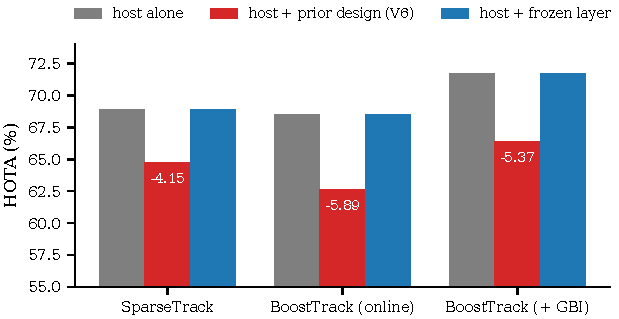
\includegraphics[width=0.7\textwidth]{figures/ch5_fig2_v6_to_v7.pdf}
\caption{The design problem: the prior always-intervening design degraded strong published trackers on MOT17 (difference in white); the frozen layer leaves them at their own accuracy.}
\label{fig:ch5-v6}
\end{figure}

\begin{table}[tbp]
\centering
\caption{Design steps from the prior always-intervening design to the frozen policy (development data, HOTA \%), and variants tested and rejected.}
\label{tab:ch5-ablation}
\small\setlength{\tabcolsep}{4pt}
\begin{adjustbox}{max width=\textwidth}
\begin{tabular}{>{\raggedright\arraybackslash}p{3.1cm}>{\raggedright\arraybackslash}p{4.8cm}>{\raggedright\arraybackslash}p{6.9cm}}
\hline
Step & Change & Effect \\
\hline
V6 emulated inside V7 & always-noisy bands, overlap deduplication, rank remap & ByteTrack (0.1) 56.41 vs host 67.70; OC-SORT (0.1) 45.72 vs 66.44 \\
V7a--V7d & regime statistic, host-anchored clean regime, crowd-safe duplicates & SparseTrack 64.72 to 68.93 (host 68.88); BoostTrack 62.61 to 68.37 (host 68.49) \\
+ whole-stream regime & regime from all past frames & ByteTrack (0.1) 67.561 to 67.702; OC-SORT (0.1) 65.697 to 66.071 \\
+ continuation rescue & foreground track-consistent rescue & OC-SORT (0.01) 66.405 to 66.619; OC-SORT (0.1) 66.071 to 66.469 \\
+ interpretability check = V7f & no background mode gives no evidence against the host & ByteTrack/BoostTrack (0.1) identical to host; OC-SORT 67.041 (0.01), 66.907 (0.1) \\
\hline
\multicolumn{2}{l}{\textit{Rejected variant}} & \textit{Evidence} \\
\multicolumn{2}{>{\raggedright\arraybackslash}p{8.0cm}}{no candidates at frame 1} & -0.3 to -0.5 HOTA on every MOT17 host \\
\multicolumn{2}{>{\raggedright\arraybackslash}p{8.0cm}}{rescue below a two-stage host's low stage} & FP +700 to +1000, -0.4 to -0.5 HOTA \\
\multicolumn{2}{>{\raggedright\arraybackslash}p{8.0cm}}{rank-remapped scores in clean frames} & ByteTrack -0.2 / -1.6 HOTA \\
\multicolumn{2}{>{\raggedright\arraybackslash}p{8.0cm}}{host-clipped noisy primary band} & KITTI YOLOv8n ByteTrack +1.4 HOTA but uncontrolled false tracks on a noisy aerial stream (26.9 vs 14.9 boxes/frame) \\
\hline
\end{tabular}
\end{adjustbox}
\end{table}


\subsection{Freeze and evaluation roles}
The final configuration was frozen before any external evaluation, recorded in a version-control tag, and protected by a lock file of cryptographic hashes of the layer, its configuration, and the evaluation runners; every post-freeze run verified the lock before running. Sixty-one automated tests check causality, state reset, pass-through on clean streams, independence from names, invariance to affine score transforms where designed, and lock integrity. Table~\ref{tab:ch5-data} lists the evaluation cells and their roles. Development cells (MOT17 with four trackers, KITTI with three trackers and two detectors, score-transform stress tests) were visible during design, so their gains are measured but not held out. The predeclared external systems (PD-SORT, Hybrid-SORT) were selected and declared before they were run, and run once. The post-freeze external systems (C-TWiX, TrackTrack, TOPICTrack) were selected under a protocol registered before any run, which fixed the host contracts, the reproduction criteria, and predictions of the layer's effect; a system entered the analysis only if its baseline reproduced the authors' number (EXACT: within 0.2 HOTA; CLOSE: within 1.0 with a documented, untuned cause).

\begin{table}[tbp]
\centering
\caption{Evaluation cells and their role. Development cells were visible while the layer was designed; predeclared and post-freeze cells were run once with the frozen policy.}
\label{tab:ch5-data}
\small\setlength{\tabcolsep}{4pt}
\begin{adjustbox}{max width=\textwidth}
\begin{tabular}{>{\raggedright\arraybackslash}p{3.0cm}>{\raggedright\arraybackslash}p{3.6cm}>{\raggedright\arraybackslash}p{4.6cm}>{\raggedright\arraybackslash}p{3.2cm}}
\hline
Data & Detector & Trackers & Role \\
\hline
MOT17 val-half (7 sequences) & published YOLOX-X detections & ByteTrack (2 settings), OC-SORT, BoostTrack, SparseTrack & development \\
KITTI tracking training (21 sequences) & YOLOv8n, RT-DETR-L & ByteTrack, BoT-SORT, OC-SORT & development (detector transfer) \\
MOT17 val-half, score transforms & published YOLOX-X, transformed scores & ByteTrack (2 settings), OC-SORT, BoostTrack & development (robustness) \\
MOT17 val-half & released PD-SORT / Hybrid-SORT detections & PD-SORT, Hybrid-SORT & predeclared external \\
MOT17 val-half, KITTI MOTS val (9 sequences), DanceTrack val (25 sequences) & authors' released detections & C-TWiX, TrackTrack (DanceTrack), TOPICTrack (MOT17) & post-freeze external \\
\hline
\end{tabular}
\end{adjustbox}
\end{table}


\subsection{Statistics}
All comparisons are paired: both arms use the same detections and the same environment. Differences are pooled over sequences and their 95\% intervals come from a percentile bootstrap over sequences with 10,000 resamples and seed 42 \cite{efron1993bootstrap}. A difference is called significant only when its interval excludes zero. Per-sequence wins, ties ($|\Delta\mathrm{HOTA}|<0.01$), and losses are reported as a distribution-free complement. Evaluation uses TrackEval (commit 12c8791) with the official ground truth of each benchmark.

\section{Tracker Transfer}\label{sec:ch5-tracker}
Table~\ref{tab:ch5-mot17} gives the development trackers on MOT17 val-half with the published YOLOX-X detections, and Fig.~\ref{fig:ch5-forest} summarizes every cell of the chapter.

\begin{sidewaystable}
\centering
\caption{Development hosts on MOT17 val-half (published YOLOX-X detections). Host = our reproduction; $\Delta$ = host with the frozen layer minus host, with 95\% paired-bootstrap interval (10,000 resamples, seed 42); bold intervals exclude zero. The floor is the lowest detector score emitted.}
\label{tab:ch5-mot17}
\small\setlength{\tabcolsep}{4pt}
\begin{adjustbox}{max width=\textheight}
\begin{tabular}{llllccc}
\hline
Tracker & Setting & Paper HOTA / MOTA / IDF1 & Host HOTA / MOTA / IDF1 & $\Delta$HOTA & $\Delta$MOTA & $\Delta$IDF1 \\
\hline
SparseTrack & -- & 69.2 / 76.8 / 81.4 & 68.88 / 77.85 / 81.97 & $+0.06$ [$-0.01$, $+0.25$] & $+0.08$ [$-0.03$, $+0.30$] & $+0.16$ [$-0.01$, $+0.70$] \\
BoostTrack & online & 68.37 / 75.56 / 81.35 & 68.49 / 75.50 / 81.41 & 0 (identical) & 0 (identical) & 0 (identical) \\
BoostTrack & + GBI & 71.33 / 80.55 / 83.84 & 71.72 / 81.03 / 84.16 & 0 (identical) & 0 (identical) & 0 (identical) \\
ByteTrack & floor 0.01 & -- / 76.6 / 79.3 & 67.70 / 77.60 / 79.47 & $-0.014$ [$-0.058$, $+0.009$] & $+0.06$ [$-0.15$, $+0.34$] & $-0.03$ [$-0.14$, $+0.04$] \\
ByteTrack & floor 0.1 & -- / 76.6 / 79.3 & 67.70 / 77.60 / 79.47 & 0 (identical) & 0 (identical) & 0 (identical) \\
OC-SORT & floor 0.01 & 66.5 / 74.9 / 77.7 & 66.43 / 74.67 / 78.05 & {\boldmath $+0.61$ [$+0.36$, $+1.24$]} & {\boldmath $+1.27$ [$+0.17$, $+3.01$]} & $+0.66$ [$-0.25$, $+1.60$] \\
OC-SORT & floor 0.1 & 66.5 / 74.9 / 77.7 & 66.44 / 74.67 / 78.05 & {\boldmath $+0.46$ [$+0.27$, $+1.09$]} & {\boldmath $+1.26$ [$+0.37$, $+3.34$]} & {\boldmath $+0.287$ [$+0.003$, $+0.838$]} \\
\hline
\end{tabular}
\end{adjustbox}
\end{sidewaystable}


\begin{figure}[tbp]
\centering
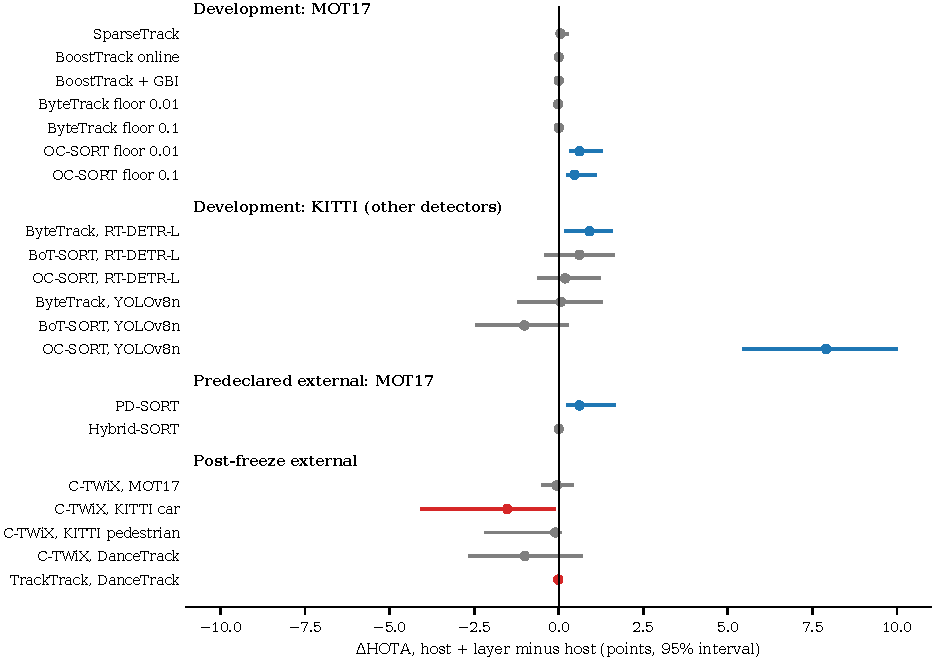
\includegraphics[width=0.92\textwidth]{figures/ch5_fig3_forest.pdf}
\caption{Every evaluated cell: difference in HOTA (tracker with the frozen layer minus tracker alone) with 95\% paired-bootstrap interval. Blue: interval above zero; red: below zero; gray: includes zero or identical output.}
\label{fig:ch5-forest}
\end{figure}

The two-stage trackers with well-matched detections were left unchanged. BoostTrack (online and with interpolation) and ByteTrack at floor 0.1 produced identical output; ByteTrack at floor 0.01 changed by $-0.014$ ($[-0.058,+0.009]$); SparseTrack changed by $+0.055$ ($[-0.011,+0.254]$). This is the intended self-limiting behavior, and it is the result the prior design could not achieve (Fig.~\ref{fig:ch5-v6}).

The single-stage OC-SORT improved at both emission floors: HOTA $+0.61$ ($[+0.36,+1.24]$) and $+0.46$ ($[+0.27,+1.09]$), MOTA $+1.27$ and $+1.26$, with gains on 7 of 7 sequences in both settings (Fig.~\ref{fig:ch5-perseq}). The mechanism is the continuation rescue: OC-SORT discards every detection below its single threshold, and the layer hands it the foreground candidates that continue an unmatched track.

\begin{figure}[tbp]
\centering
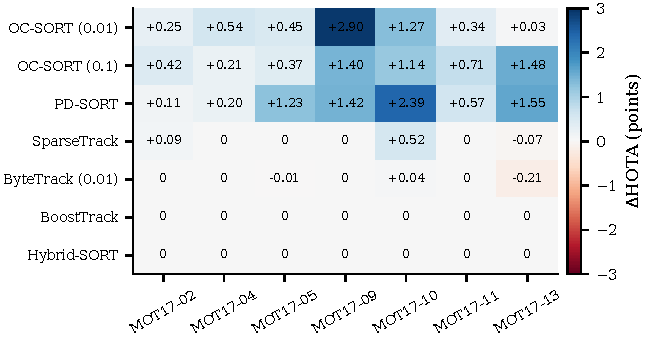
\includegraphics[width=0.7\textwidth]{figures/ch5_fig4_per_sequence.pdf}
\caption{Per-sequence HOTA differences on MOT17 val-half for development and predeclared trackers.}
\label{fig:ch5-perseq}
\end{figure}

\section{Detector Transfer}\label{sec:ch5-detector}

\subsection{A different detector and dataset}
On KITTI tracking training, three trackers were run with two detectors other than the MOT17 detector (Table~\ref{tab:ch5-kitti}). With the noisy RT-DETR-L stream \cite{zhao2024rtdetr}, the two-stage trackers gained substantially in MOTA and IDF1: ByteTrack $+5.98$ MOTA ($[+1.16,+9.94]$) and $+3.87$ IDF1, BoT-SORT $+7.86$ MOTA ($[+2.21,+13.44]$) and $+3.10$ IDF1, with HOTA $+0.91$ ($[+0.22,+1.55]$) for ByteTrack. With YOLOv8n, the single-stage OC-SORT gained 7.91 HOTA ($[+5.47,+9.98]$), while ByteTrack and BoT-SORT lost MOTA ($-1.87$ and $-2.43$, the latter significant) while their identity switches fell by about half; this regression is analyzed in Sec.~\ref{sec:ch5-failures}.

\begin{sidewaystable}
\centering
\caption{Detector transfer on KITTI tracking training (official HOTA, car and pedestrian averaged). BoT-SORT excludes one sequence on which the unmodified tracker fails numerically.}
\label{tab:ch5-kitti}
\small\setlength{\tabcolsep}{4pt}
\begin{adjustbox}{max width=\textheight}
\begin{tabular}{llcccc}
\hline
Tracker & Detector & Host HOTA / MOTA / IDF1 & $\Delta$HOTA & $\Delta$MOTA & $\Delta$IDF1 \\
\hline
ByteTrack & RT-DETR-L & 50.73 / 47.27 / 64.98 & {\boldmath $+0.91$ [$+0.22$, $+1.55$]} & {\boldmath $+5.98$ [$+1.16$, $+9.94$]} & {\boldmath $+3.87$ [$+1.67$, $+5.06$]} \\
BoT-SORT & RT-DETR-L & 53.91 / 48.25 / 67.74 & $+0.61$ [$-0.39$, $+1.61$] & {\boldmath $+7.86$ [$+2.21$, $+13.44$]} & {\boldmath $+3.10$ [$+1.00$, $+4.57$]} \\
OC-SORT & RT-DETR-L & 52.64 / 57.59 / 69.87 & $+0.19$ [$-0.57$, $+1.19$] & $-0.57$ [$-4.36$, $+1.40$] & $+0.04$ [$-1.31$, $+1.78$] \\
ByteTrack & YOLOv8n & 45.31 / 46.54 / 60.92 & $+0.06$ [$-1.19$, $+1.24$] & $-1.87$ [$-6.25$, $+0.03$] & $+1.49$ [$-0.36$, $+3.27$] \\
BoT-SORT & YOLOv8n & 49.21 / 49.89 / 64.41 & $-1.02$ [$-2.43$, $+0.25$] & {\boldmath $-2.43$ [$-7.43$, $-0.14$]} & $+0.35$ [$-2.10$, $+2.27$] \\
OC-SORT & YOLOv8n & 36.27 / 33.99 / 50.46 & {\boldmath $+7.91$ [$+5.47$, $+9.98$]} & {\boldmath $+9.40$ [$+1.10$, $+12.30$]} & {\boldmath $+9.60$ [$+5.61$, $+12.16$]} \\
\hline
\end{tabular}
\end{adjustbox}
\end{sidewaystable}


\subsection{Detector confidence shift}
To isolate the calibration problem, the published MOT17 detections were transformed before the tracker by four monotone maps: cubing ($s^3$), halving ($0.5s$), and logit temperatures 2 and 0.5 (Fig.~\ref{fig:ch5-shift}). The trackers kept their published thresholds. Halving the scores drove ByteTrack (official setting) and OC-SORT to 0 HOTA because no detection reached their thresholds; with the layer they reached 66.17 and 66.72. Cubing reduced them to 60.92 and 58.34; with the layer they reached 65.81 and 66.60, and BoostTrack went from 61.33 to 64.84. Under the temperatures the layer gained up to 1.23 points or left the output unchanged. The ByteTrack library setting, whose low thresholds already admit the shifted scores, was unchanged within 0.14 points in all four transforms. These cells are development evidence. Their paired intervals were computed after the freeze on the recorded runs, whose replay reproduced every recorded metric exactly (Table~\ref{tab:ch5-shiftboot}): the layer recovered significantly in 7 of the 14 conditions and degraded significantly in none, and the other 7 were identical or had intervals including zero.

\begin{table}[tbp]
\centering
\caption{Detector confidence shift on MOT17 val-half with 95\% paired-bootstrap intervals (10,000 resamples, seed 42), computed after the freeze on the recorded runs. HOTA of each tracker with its published thresholds, alone and with the frozen layer; bold intervals exclude zero; W/T/L are per-sequence wins, ties, and losses.}
\label{tab:ch5-shiftboot}
\small\setlength{\tabcolsep}{4pt}
\begin{adjustbox}{max width=\textwidth}
\begin{tabular}{llrrlc}
\hline
Tracker (setting) & Transform & Alone & With layer & $\Delta$HOTA & W/T/L \\
\hline
ByteTrack (official setting) & $s^3$ & 60.92 & 65.81 & {\boldmath $+4.89$ [$+2.60$, $+13.69$]} & 7/0/0 \\
ByteTrack (official setting) & $0.5s$ & 0.00 & 66.17 & {\boldmath $+66.17$ [$+49.32$, $+75.40$]} & 7/0/0 \\
ByteTrack (official setting) & temperature 2 & 65.84 & 66.95 & {\boldmath $+1.11$ [$+0.35$, $+3.87$]} & 6/0/1 \\
ByteTrack (official setting) & temperature 0.5 & 67.30 & 67.29 & $-0.01$ [$-0.05$, $+0.00$] & 1/4/2 \\
ByteTrack (library setting) & $s^3$ & 66.31 & 66.31 & $-0.01$ [$-0.38$, $+0.38$] & 3/0/4 \\
ByteTrack (library setting) & $0.5s$ & 66.61 & 66.48 & $-0.14$ [$-0.66$, $+0.14$] & 2/3/2 \\
ByteTrack (library setting) & temperature 2 & 63.97 & 63.97 & 0 (identical) & 0/7/0 \\
ByteTrack (library setting) & temperature 0.5 & 66.53 & 66.52 & $-0.01$ [$-0.03$, $+0.00$] & 0/5/2 \\
OC-SORT & $s^3$ & 58.34 & 66.60 & {\boldmath $+8.26$ [$+5.86$, $+16.81$]} & 7/0/0 \\
OC-SORT & $0.5s$ & 0.00 & 66.72 & {\boldmath $+66.72$ [$+50.32$, $+75.56$]} & 7/0/0 \\
OC-SORT & temperature 2 & 65.99 & 67.22 & {\boldmath $+1.24$ [$+0.52$, $+3.42$]} & 6/0/1 \\
OC-SORT & temperature 0.5 & 66.61 & 67.06 & $+0.45$ [$-0.01$, $+0.97$] & 4/0/3 \\
BoostTrack online & $s^3$ & 61.33 & 64.84 & {\boldmath $+3.51$ [$+0.85$, $+13.28$]} & 7/0/0 \\
BoostTrack online & temperature 2 & 67.59 & 67.59 & 0 (identical) & 0/7/0 \\
\hline
\end{tabular}
\end{adjustbox}
\end{table}


\begin{figure}[tbp]
\centering
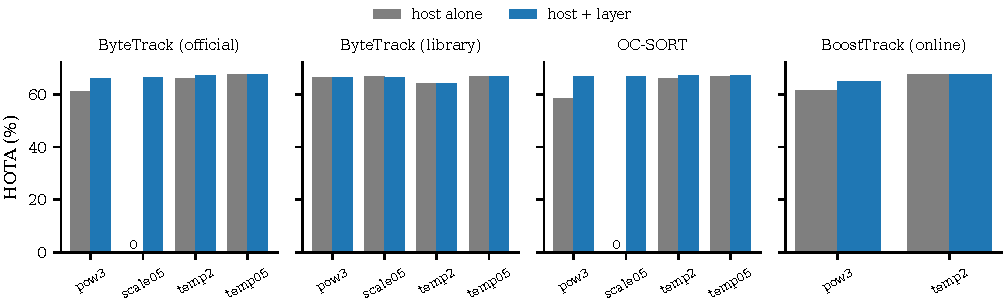
\includegraphics[width=\textwidth]{figures/ch5_fig5_calibration_shift.pdf}
\caption{Detector confidence shift on MOT17 val-half: HOTA of each published tracker with its published thresholds, alone and with the frozen layer, after four monotone transforms of the detector scores.}
\label{fig:ch5-shift}
\end{figure}

\section{Post-Freeze External Evaluation}\label{sec:ch5-external}
Table~\ref{tab:ch5-external} gives every external system evaluated with the frozen layer.

\begin{sidewaystable}
\centering
\caption{External systems evaluated once with the frozen layer. Reproduction class against the authors' reported number (EXACT: $|\Delta\mathrm{HOTA}|\le0.2$; CLOSE: $\le1.0$ with a documented, untuned cause). TOPICTrack failed reproduction and is excluded from the analysis.}
\label{tab:ch5-external}
\small\setlength{\tabcolsep}{4pt}
\begin{adjustbox}{max width=\textheight}
\begin{tabular}{llllccc}
\hline
System & Data & Reference / reproduced HOTA & Class & $\Delta$HOTA & $\Delta$MOTA & $\Delta$IDF1 \\
\hline
\multicolumn{7}{l}{\textit{Predeclared before the runs}}\\
PD-SORT & MOT17 val-half & 68.01 / 68.01 & EXACT (released output) & {\boldmath $+0.61$ [$+0.27$, $+1.65$]} & {\boldmath $+1.13$ [$+0.27$, $+3.03$]} & {\boldmath $+0.82$ [$+0.43$, $+1.94$]} \\
Hybrid-SORT & MOT17 val-half & 67.1 / 66.70 & CLOSE & 0 (identical) & 0 (identical) & 0 (identical) \\
\multicolumn{7}{l}{\textit{Post-freeze, protocol registered before the runs}}\\
C-TWiX & MOT17 val-half & 77.8 / 77.55 & CLOSE & $-0.05$ [$-0.46$, $+0.40$] & $+0.24$ [$-0.58$, $+1.12$] & $+0.18$ [$-0.47$, $+1.14$] \\
C-TWiX (car) & KITTI MOTS val & 89.3 / 89.27 & EXACT & {\boldmath $-1.52$ [$-4.05$, $-0.13$]} & {\boldmath $-2.11$ [$-5.89$, $-0.17$]} & {\boldmath $-1.21$ [$-3.32$, $-0.10$]} \\
C-TWiX (pedestrian) & KITTI MOTS val & 71.4 / 70.77 & CLOSE & $-0.10$ [$-2.16$, $+0.03$] & $-0.31$ [$-4.86$, $+0.10$] & $-0.01$ [$-1.90$, $+0.08$] \\
C-TWiX & DanceTrack val & 60.4 / 59.62 & CLOSE & $-1.00$ [$-2.62$, $+0.65$] & $+0.13$ [$-0.39$, $+0.47$] & $-1.55$ [$-3.76$, $+0.52$] \\
TOPICTrack & MOT17 val-half & 69.6 / 67.54 & FAILED & \multicolumn{3}{c}{not analyzed} \\
TrackTrack & DanceTrack val & 63.3 / 62.96 & CLOSE & {\boldmath $-0.013$ [$-0.032$, $-0.001$]} & {\boldmath $-0.073$ [$-0.208$, $-0.004$]} & $+0.009$ [$-0.001$, $+0.028$] \\
\hline
\end{tabular}
\end{adjustbox}
\end{sidewaystable}


\subsection{Predeclared systems}
PD-SORT \cite{wang2025pdsort} was reproduced identically to the authors' released output. With the layer, HOTA rose by 0.61 ($[+0.27,+1.65]$), MOTA by 1.13 ($[+0.27,+3.03]$), and IDF1 by 0.82 ($[+0.43,+1.94]$), with HOTA higher on 7 of 7 sequences (Fig.~\ref{fig:ch5-perseq}). False negatives fell by 1,291 and false positives rose by 681. PD-SORT is single-stage, and the gain follows the same mechanism as for OC-SORT; unlike OC-SORT, PD-SORT was not seen during design. Hybrid-SORT \cite{yang2024hybridsort}, a two-stage tracker, produced identical output, as predicted.

\subsection{Recent systems after the freeze}
C-TWiX \cite{miah2025twix} was reproduced on three datasets (Table~\ref{tab:ch5-external}). On MOT17 the layer changed HOTA by $-0.05$ ($[-0.46,+0.40]$) with MOTA $+0.24$ and IDF1 $+0.18$; on KITTI pedestrians by $-0.10$ ($[-2.16,+0.03]$); on DanceTrack by $-1.00$ ($[-2.62,+0.65]$) with an IDF1 loss of 1.55 whose interval includes zero. On KITTI cars it lost 1.52 HOTA ($[-4.05,-0.13]$), the one significant external degradation of the paper (Sec.~\ref{sec:ch5-failures}). TrackTrack \cite{shim2025tracktrack} was reproduced within 0.34 HOTA on DanceTrack; the layer changed its HOTA by $-0.013$ ($[-0.032,-0.001]$), a significant but negligible difference, with 21 of 25 sequences tied. TOPICTrack \cite{cao2025topictrack} failed the registered reproduction criterion (67.54 against 69.6 HOTA) and is excluded; the frozen layer's effect on it ($-0.016$, interval including zero) is recorded but not analyzed.

\section{Cross-Dataset Analysis}\label{sec:ch5-cross}
Across MOT17, KITTI, and DanceTrack, the direction of the effect is predicted by two properties of the pipeline rather than by the dataset: whether the tracker has a continuation stage and whether the detector's score distribution matches the tracker's thresholds. The regime estimate makes this visible (Fig.~\ref{fig:ch5-regimes}a): on the post-freeze streams, 99.7\% of MOT17 frames and 99.9\% of DanceTrack frames were classified clean, and the layer left those pipelines at or near their native output. KITTI had the largest noisy share (2.8\% of frames), concentrated in short sequences.

\begin{figure}[tbp]
\centering
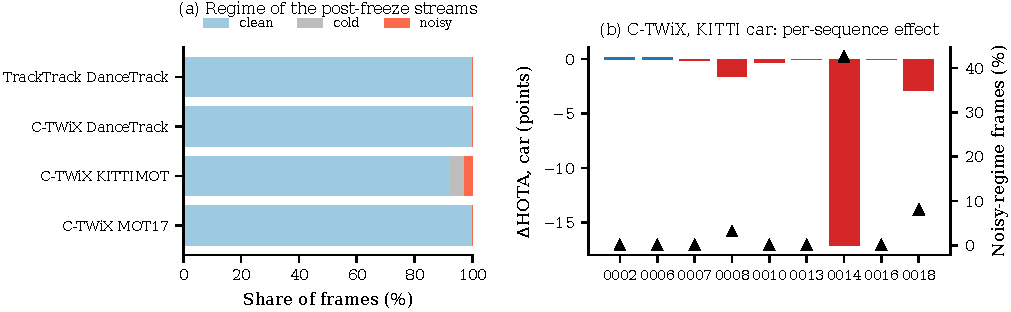
\includegraphics[width=\textwidth]{figures/ch5_fig6_regimes_failure.pdf}
\caption{(a) Share of frames in each regime on the post-freeze streams. (b) C-TWiX on KITTI cars: per-sequence HOTA difference (bars) and share of frames classified noisy (triangles); the loss concentrates in sequence 0014.}
\label{fig:ch5-regimes}
\end{figure}

\section{Robustness Analysis}\label{sec:ch5-robust}
Three kinds of robustness were measured. Score transforms (Sec.~\ref{sec:ch5-detector}) test calibration shift with the detections fixed; the worst cell was $-0.14$ HOTA, with an interval including zero. Emission floors test how much of the low-score tail the detector emits: on MOT17 the two-stage trackers were unchanged at floors 0.01 and 0.1, and OC-SORT improved at both. Detector changes test both at once: RT-DETR-L on KITTI produced the largest MOTA and IDF1 gains for two-stage trackers, and YOLOv8n produced the regression analyzed next. The emission floor is also the design's largest label-free sensitivity: in development diagnostics of an earlier variant on aerial video, raising the floor to 0.2 changed the regime of 41--45\% of frames, because the pooled statistics move with the floor.

\section{Ablation}\label{sec:ch5-ablation}
Table~\ref{tab:ch5-ablation} traces the design from the always-intervening layer to the frozen configuration on development data. Emulating the prior design inside the new framework reduced ByteTrack at floor 0.1 from 67.70 to 56.41 HOTA and OC-SORT from 66.44 to 45.72. The regime estimate with the self-limiting clean regime and crowd-safe duplicates restored SparseTrack from 64.72 to 68.93 and BoostTrack from 62.61 to 68.37. Estimating the regime from the whole stream removed mid-stream flips, the continuation rescue added 0.2--0.4 points for OC-SORT, and the interpretability check returned ByteTrack and BoostTrack to identical-to-host output while raising OC-SORT to 67.04 and 66.91. Four variants were rejected on evidence: admitting nothing at the first frame, rescuing below a two-stage tracker's low stage, remapping scores in clean frames, and clipping the noisy primary band to the host threshold, which helped one KITTI cell but let a noisy aerial stream produce 26.9 instead of 14.9 boxes per frame.

\section{Statistical Analysis}\label{sec:ch5-stats}
Of the 16 cells in Fig.~\ref{fig:ch5-forest} with an interval, 7 exclude zero in HOTA: 5 above zero (OC-SORT twice on MOT17, OC-SORT with YOLOv8n and ByteTrack with RT-DETR-L on KITTI, and PD-SORT) and 2 below (C-TWiX on KITTI cars, $-1.52$, and TrackTrack, $-0.013$). Four further cells produced identical output. In MOTA, significant gains occurred for OC-SORT on MOT17 and with YOLOv8n, PD-SORT, and ByteTrack and BoT-SORT with RT-DETR-L, and significant losses for BoT-SORT with YOLOv8n, C-TWiX on KITTI cars, and TrackTrack ($-0.073$). The external evidence is therefore mixed in sign and small in magnitude except for the single-stage PD-SORT, whose gain is the only external improvement with every interval above zero. The intervals are per-cell and descriptive, without correction for multiple comparisons; with 16 cells, about one could exclude zero by chance, which is one more reason to read the external evidence as mixed. With 7, 9, or 25 sequences per cell, the intervals are wide, and differences below a few tenths of a point in HOTA are not resolved except when the output is nearly identical.

\section{Runtime}\label{sec:ch5-runtime}
Table~\ref{tab:ch5-runtime} and Fig.~\ref{fig:ch5-runtime} give the cost on a four-core Intel Xeon processor without a graphics processor, with a live YOLOv8n detector and ByteTrack on three KITTI sequences. The layer took 2.95 ms per frame on average (4.39 ms at the 95th percentile), including the phase-correlation motion cue. End-to-end time rose from 57.85 to 60.44 ms per frame (4.5\%), and the tracker became faster (2.04 to 1.43 ms) because it received fewer candidates. On this processor the full pipeline ran at 16.55 frames per second, below real time, because the detector dominates; no throughput is claimed for other hardware.

\begin{table}[tbp]
\centering
\caption{Per-frame time on a 4-vCPU Intel Xeon (2.10 GHz, no graphics processor), live YOLOv8n (736 pixels) and ByteTrack on three KITTI sequences (2,279 timed frames per arm), mean / 95th percentile in milliseconds.}
\label{tab:ch5-runtime}
\small\setlength{\tabcolsep}{4pt}
\begin{adjustbox}{max width=\textwidth}
\begin{tabular}{lcc}
\hline
Stage & Host alone & Host + V7f \\
\hline
Frame decode & 13.88 / 16.21 & 13.88 / 16.51 \\
Detector (YOLOv8n, 736 px) & 41.91 / 58.41 & 42.17 / 59.43 \\
AC-MOT controller & -- & 2.95 / 4.39 \\
Tracker (ByteTrack) & 2.04 / 3.57 & 1.43 / 2.64 \\
End to end & 57.85 / 76.35 & 60.44 / 80.78 \\
\hline
\end{tabular}
\end{adjustbox}
\end{table}


\begin{figure}[tbp]
\centering
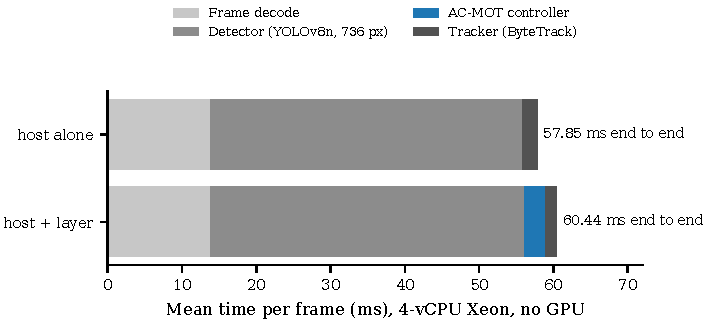
\includegraphics[width=0.66\textwidth]{figures/ch5_fig7_runtime.pdf}
\caption{Mean per-frame time by stage without and with the layer.}
\label{fig:ch5-runtime}
\end{figure}

\section{Failure Cases}\label{sec:ch5-failures}

\subsection{False noisy calls in short streams}
The significant external loss, C-TWiX on KITTI cars ($-1.52$ HOTA), is concentrated in one sequence: in sequence 0014 the layer classified 45 of 106 frames as noisy and HOTA fell by 17.09 points, while six of the other eight sequences changed by less than 0.4 points (Fig.~\ref{fig:ch5-regimes}b). In this short sequence the whole-stream median of $\rho$ had little history to stabilize it, and the noisy regime's band restrictions most likely removed detections that the coordinate-based association relies on; the mechanism was not isolated further. The same sequence accounts for the pedestrian loss (8.50 points). A cold-start protection that requires a minimum amount of history before a noisy call is a natural remedy, but it was not part of the frozen configuration and is left to future work.

\subsection{Under-confident detectors with low-threshold trackers}
With YOLOv8n on KITTI, whose scores are low but mostly correct, the stream is classified noisy ($\rho\approx0.45$), and the noisy regime's rule that only the primary band may start tracks removes true births for ByteTrack and BoT-SORT. MOTA fell by 1.87 and 2.43 while identity switches fell by 271 and 227. A host-relative band that fixed this cell let false tracks through on a noisy aerial stream and was rejected (Table~\ref{tab:ch5-ablation}).

\subsection{Coordinate-only association on DanceTrack}
C-TWiX on DanceTrack lost 1.00 HOTA with an interval including zero, with two sequences losing more than 10 points and one gaining 9.37. The regime was clean on essentially every frame, so the effect comes from the clean-regime operations (cross-class duplicate removal, threshold lowering to $t_2$, and the continuation rescue) acting on a tracker that learns association from coordinates; which of them causes the loss was not isolated.

\section{Limitations}\label{sec:ch5-limits}
\begin{enumerate}
\item The strongest evidence is development evidence. Only PD-SORT, Hybrid-SORT, C-TWiX, and TrackTrack are external, and only PD-SORT improved.
\item No head-to-head comparison with per-frame adaptive-threshold trackers \cite{ma2023adaptivebytetrack,shim2024adaptrack,act2026adaptive} was run. The closest baseline evaluated is the always-intervening prior design, which uses the same score statistics in every frame without a regime decision (Table~\ref{tab:ch5-ablation}).
\item The external systems were evaluated on validation splits with the authors' released detections; no test-server result is reported.
\item The motion rule could not be evaluated on the external systems, whose adapters had no image cue.
\item The aerial evaluation planned for the frozen layer could not be completed because the benchmark data could not be downloaded in the evaluation environment; no aerial claim is therefore made for the frozen layer.
\item Runtime was measured on one general-purpose processor without a graphics processor; no embedded or flight hardware was tested.
\item Reproductions on processors instead of graphics processors differ from the authors' numbers by up to 0.8 HOTA; all comparisons are paired within one environment.
\end{enumerate}

\section{Summary}\label{sec:ch5-conclusions}
This chapter presented a training-free control layer that self-calibrates from a detector's score stream, estimates whether the stream is clean or noisy, and adapts a frozen tracker's input and thresholds through a declared host contract. One frozen configuration was evaluated on nine published trackers, four sources of detections, and three datasets, with development and external evidence kept separate. The layer improved single-stage trackers, including a predeclared external one by 0.61 HOTA points; it restored trackers whose thresholds no longer matched a shifted detector confidence scale; and it raised the multi-object tracking accuracy of two-stage trackers with a noisy detector by 6 to 8 points. On well-matched two-stage pipelines it left the output unchanged, which removed the degradation of the prior design. It failed on a short stream with few candidates, where false noisy calls cost one external tracker 1.52 HOTA points, and on an under-confident detector with low-threshold trackers. For tracking pipelines in which detectors are exchanged more often than trackers are retuned, the layer provides a way to keep published trackers operating without labelled recalibration, together with an explicit record of where it should not be expected to help.

